\section{Entwurf}

\subsection{Kommunikationseinheit} \label{commModule}

\subsubsection{init/0}

Beim Initialisieren einer Kommunikationseinheit wird ein Prozess gestartet, welcher beim \textit{towerCBC} registriert wird und bei der \textit{towerClock} eine neue Vektoruhr ID anfragt. Wie in Abb. \ref{fig:sequence_cbCast_init} zu sehen, wird der Aufruf an die \textit{towerClock} von dem Prozess gesendet, der auch beim \textit{towerCBC} registriert wird. Grund dafür ist, dass die \textit{towerClock} die Prozess ID des anfragenden Prozesses auf dessen Vektoruhr ID mappt. Würde der Prozess, welcher den \textit{cbCast} Prozess erzeugt diese Anfrage schicken, würde dieses Mapping eine falsche Prozess ID speichern.
\\Der Verbindungsaufbau oder auch Verbindungstest terminiert das Programm, wenn er fehlschlägt.
\\Nach Erzeugung des \textit{cbCast} Prozesses ist dieser sequenziell nicht mehr gebunden an den Prozess, der diesen erzeugt hat. Dementsprechend verlaufen die Aufrufe dieser beiden Nebenläufig.

\begin{figure}[htbp]
\begin{center}
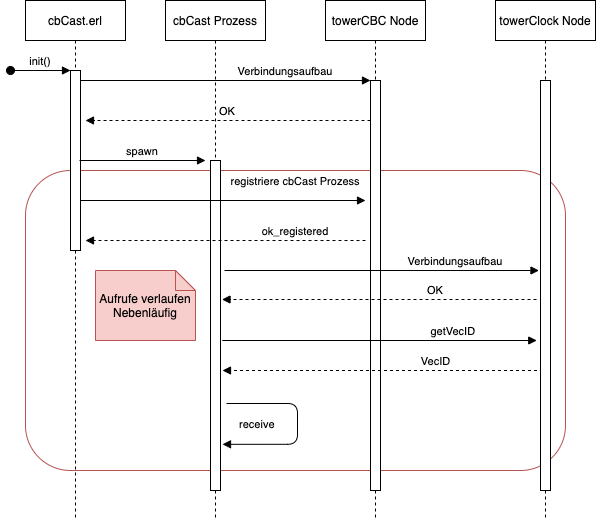
\includegraphics[scale=0.55]{Latex/Bilder/Sequenzdiagramm_cbCast.png}
\caption{\label{fig:sequence_cbCast_init} Sequenzdiagramm Initialisierung}
\end{center}
\end{figure}

Alternativ könnte sich der \textit{cbCast.erl} auch erst beim \textit{towerClock} die \textit{VektorID} holen und dann den \textit{cbCast} Prozess erzeugen. Durch den Ablauf in Abb. \ref{fig:sequence_cbCast_init} kann das holen der \textit{VektorID} aber nebenläufig zur Registrierung beim \textit{towerCBC} passieren. Der ganze Vorgang ist somit schneller.

\subsubsection{stop/1}

Die Terminierung erfolgt auf zwei verschiedene Wege. Zuerst wird der Prozess gestoppt, das bedeutet das eine sogenannter \textit{Graceful Shutdown} durchgeführt wird. Hat dieser kein Erfolg wird der Prozess durch einen \textit{Hard Shutdown} gekillt.\\
Als Parameter wird der zu terminierende Prozess übergeben.

\subsubsection{send/2}

Beim Senden (siehe Abb. \ref{fig:sequence_cbCast_send}) wird eine Nachricht \textit{(Msg)} an den als Parameter übergebenen \textit{Kommunikationsprozess (cbCast Prozess)} geschickt. Dieser erhöht seine Vektoruhr vor dem Senden um 1 und verschickt die Nachricht an den \textit{Multicast}. Der \textit{Multicast} verteilt die Nachricht an alle Prozesse, inklusive dem Sender.\\
Die Vektoruhr der versendeten Nachricht hat zu der Vektoruhr der \textit{Kommunikationseinheit} eine Distanz von -1, wodurch diese Nachricht auslieferbar ist und direkt in die \textit{Delivery Queue} einsortiert werden könnte.
Wenn die gesendete Nachricht vom \textit{Multicast} empfangen wird, wird diese dennoch zuerst in die \textit{Holdback Queue} einsortiert um eine kausale Ordnung zu garantieren.

\begin{figure}[htbp]
\begin{center}
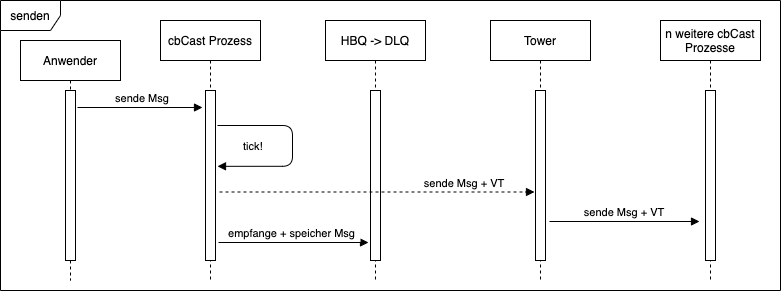
\includegraphics[scale=0.5]{Latex/Bilder/Sequenz_senden.png}
\caption{\label{fig:sequence_cbCast_send} Sequenzdiagramm Senden}
\end{center}
\end{figure}

\subsubsection{read/1 \& received/1}

\begin{figure}[htbp]
\begin{center}
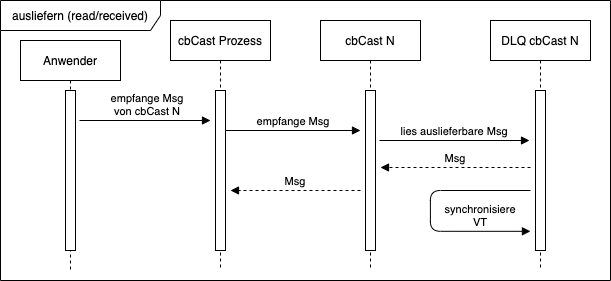
\includegraphics[scale=0.5]{Latex/Bilder/Sequenz_ausliefern.png}
\caption{\label{fig:sequence_cbCast_read_receive} Sequenzdiagramm Ausliefern}
\end{center}
\end{figure}

Das Ausliefern einer Nachrichten (siehe Abb. \ref{fig:sequence_cbCast_read_receive}) liest eine Nachricht aus der \textit{Delivery Queue} des \textit{Kommunikationsprozesses (cbCast N)}, welcher als Parameter übergeben wurde.\\
Hierfür gibt es eine Funktion, welche blockierend und eine, welche nicht blockierend empfängt.

\paragraph{read/1 (nicht blockierend)}

Falls der angefragte Prozess keine auslieferbare Nachricht zur Verfügung hat, wird nichts empfangen und der anfragende Prozess läuft normal weiter.

\paragraph{receive/1 (blockierend)}

Falls der angefragte Prozess keine auslieferbare Nachricht zur Verfügung hat, wartet der anfragende Prozess so lange, bis eine auslieferbare Nachricht empfangen wird.\\

In beiden Funktionen synchronisiert der angefragte Prozess anschließend seine Vektoruhr mit der der ausgelieferten Nachricht, falls eine Nachricht verschickt wurde.

\subsubsection{$\{\langle PID \rangle,\{castMessage,\{\langle Message \rangle, \langle VT \rangle\}\}\}$}

Wenn der \textit{Multicast (Tower)} eine Nachricht verschickt, wird diese von der Schnittstelle $\{\langle PID \rangle,\{castMessage,\{\langle Message \rangle, \langle VT \rangle\}\}\}$ der \textit{Kommunikationsprozesses} empfangen (siehe Abb. \ref{fig:sequence_cbCast_cbcast}). Daraufhin wird die Nachricht in der \textit{Holdback Queue} des Prozesses einsortiert.

\begin{figure}[htbp]
\begin{center}
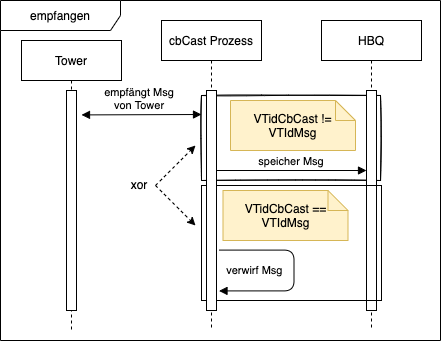
\includegraphics[scale=0.5]{Latex/Bilder/Sequenz_empfangen.png}
\caption{\label{fig:sequence_cbCast_cbcast} Sequenzdiagramm Empfangen}
\end{center}
\end{figure}

\subsubsection{Die Queues}

Sowohl die \textit{Holdback} als auch die \textit{Delivery Queue} sind Listen, welche die Nachrichten als Elemente enthalten. In der \textit{Holdback Queue} werden die Nachrichten absteigend nach den Vektoruhren der jeweiligen Nachrichten sortiert. Ist eine Nachricht \textit{after} (siehe \ref{positionVTs}) der ersten Nachricht der \textit{Holdback Queue} wird diese am Anfang einsortiert. Ist die Nachricht \textit{before} wird sie weiter mit den absteigenden Nachrichten verglichen, bis entweder das Ende der \textit{Queue} erreicht wurde oder bis die Nachricht wieder \textit{before} der an dem Index verglichenen Nachricht ist. Wenn eine Nachricht während des Einsortierens \textit{concurrent} zu einer Nachricht ist, wird sie vor dieser Nachricht einsortiert. Ist eine Nachricht \textit{equal} zu einer Nachricht in der \textit{Holdback Queue} wird sie verworfen.

\paragraph{checkQueues/3}

TODO!

\subsection{Vektoruhr-ADT}

\subsubsection{initVT/0}

\subsubsection{myVTid/1}

\subsubsection{myVTvc/1}

\subsubsection{myCount/1}

\subsubsection{foCount/2}

\subsubsection{isVT/1}

\subsubsection{syncVT/2}

\subsubsection{tickVT/1}

\subsubsection{compVT/2}

\subsubsection{aftereqVTJ/2}

\subsection{Vektoruhr Zentrale/Tower} \label{tower}

Die zentrale Vektoruhr (\textit{Tower}) verwaltet die Prozessnummern. Prozessnummern sind im Folgenden eindeutige IDs aus positiven ganzen Zahlen.

\subsection{TowerClock}

Der TowerClock implementiert eine wesentliche Schnittstelle, \textit{getVecID}. Aus Gründen der Erweiterbarkeit und Sicherheit mappt die TowerClock die Prozess ID des anfragenden Prozesses auf dessen Vektoruhr ID.
\\Die kleinste Zahl für eine Vektoruhr ID ist 0.

\subsection{Generelle Designentscheidungen}

\subsubsection{Logging}

Es wird pro Node eine generische .log Datei geben. Zum Beispiel für den Node \textit{'cbCast1@MacBook-Air-von-Kristoffer'} gibt es die Datei \textit{'cbCast1@MacBook-Air-von-Kristoffer'.log}. Dies bringt den Vorteil, dass die verschiedenen Kommunikationseinheiten - welche über die gleiche .beam Datei ausgeführt werden, aber auf verschiedenen Nodes laufen - separat voneinander geloggt werden.
\\Zum Debuggen war ein Gedanke, zusätzlich eine Logging Datei zu erstellen, in welcher alle Prozesse loggen. Hierdurch kann sequenziell nachverfolgt werden, ob die Reihenfolge der Aufrufe korrekt verläuft. Im Verlauf der Implementierung hat sich rausgestellt, dass diese Datei wenig Mehrwert bringt. Deswegen fehlt diese in der finalen Implementierung.